

\setcounter{section}{1}

\subsection{Indication sur les méthodes associées aux chaînes de caractères}

Les attributs suivants s'appliquent à des variables de type de chaîne de caractère :
\begin{itemize}
\item \pyv{.isalpha} renvoie \pyv{True} si c'est une des 26 lettres de l'alphabet et \pyv{False} sinon.
\begin{pyconsole}
'c'.isalpha()
'1'.isalpha()
\end{pyconsole}
\item \pyv{.index(x)} renvoie l'indice de la première occurrence de \pyv{x} :
\begin{pyconsole}
'hello'.index('l')
\end{pyconsole}
\item \pyv{.count(x)} renvoie le nombre d'occurrences de \pyv{x} :
\begin{pyconsole}
'hello'.count('l')
\end{pyconsole}
\end{itemize}

\subsection{Le chiffre de César}



Le \textbf{chiffrement de César} est un des tout premier code de chiffrement qui ait existé. 

La méthode est simple : il suffit de décaler toutes les lettres de l'alphabet du même nombre de lettres. 



Par exemple en choisissant un décalage de 3, le A devient le D, le B devient le E, le C devient le F et ainsi de suite. Pour la fin de l'alphabet, il suffit de revenir au début : le W devient Z, le X devient A, le Y devient B et le Z devient C. Ainsi un message comme << la metamorphose >> devient par décalage d'une lettre << mb nfubnpsqiptf >>, ce qui est incompréhensible pour le non initié.


\question{Avec des instructions python, définir trois chaînes de caractères nommées \textit{alphabet}, \textit{mess} et \textit{code} contenant respectivement les caractères de l'alphabet, un message à chiffrer (exemple << la metamorphose >>) et le message crypté (vide initialement). On se limitera à des lettres minuscules non accentuées. Les autres caractères (espaces, chiffres...) seront gardés tels quels (non chiffrés).}



\question{Comment est codé le message << franz >> avec une valeur de décalage $n=3$ ?}

\question{Écrire une fonction \pyv{def decalage(c:str, n:int) -> str:} permettant de renvoyer un caractère chiffrer avec le chiffrement de César.}

%\question{En utilisant les fonctionnalités découvertes dans la première partie, établir un algorithme permettant de chiffrer un message par le code de César, pour un décalage $n$ donné. La fonction aura la signature suivante :
%\pyv{def chiffrement_cesar(mess:str, n:int) -> str:}. }

\question{Etablir un algorithme permettant de chiffrer un message par le code de César, pour un décalage $n$ donné. La fonction associée à cet algorithme aura la signature suivante :
\pyv{def chiffrement_cesar(mess:str, n:int) -> str:}. }




\question{Proposer ensuite l'algorithme de déchiffrement qui affiche le message chiffré en clair, en supposant que $n$ est inconnu. L'utilisateur choisira parmi les déchiffrements proposés celui qui a du sens ! La fonction aura la signature suivante :
\pyv{def decryptage_cesar(code:str) -> None:}.}


%
%\question{Pouvez-vous déchiffrer ce message secret intercepté dans un couloir du lycée : {\em << xq bdaotmuz pqhaud eqdm gz egvqf pq yapqxuemfuaz >>}. Quelle est la faiblesse de ce type de code ?}

\question{Quelle est la faiblesse de ce type de code ? Proposer en deux lignes une méthode permettant de déterminer (casser) la clé.} 



\subsection{Le chiffre de Vigenère}

\begin{figure}[!htb]
\begin{minipage}{0.5\textwidth}
On étudie maintenant la méthode de chiffrement de Vigenère. Pour comprendre le système de chiffrement, on commence par créer la table  Vigenère : on recopie $26$ fois l'alphabet en ligne et à chaque saut de ligne on décale d'une lettre vers la droite comme sur la figure \ref{fig:vigenere}.

Cet algorithme fonctionne à l'aide d'une clé de chiffrement : une chaîne de caractère (typiquement un mot).

Prenons un exemple, mettons que l'on veuille coder \og anticonstitutionnellement\fg~avec la clé \og roue\fg~. Pour ce faire, on crée le tableau présenté table \ref{TabVig} dont la première ligne contient le message à coder, et la deuxième la clé répétée autant de fois que nécessaire pour atteindre la longueur du texte à coder. On fait alors une lecture colonne par colonne de ce tableau et dans chaque colonne :
\begin{enumerate}
\item la première ligne donne l'abscisse dans la table de la lettre à coder;
\item la deuxième donne l'ordonnée dans la table de la lettre à coder;
\end{enumerate}
Ainsi le chiffrement du mot \og anticonstitutionnellement\fg~ avec la clé \og roue\fg~ est obtenue dans la table \ref{TabVig}.
\end{minipage}
\begin{minipage}{0.5\textwidth}
	\centering
		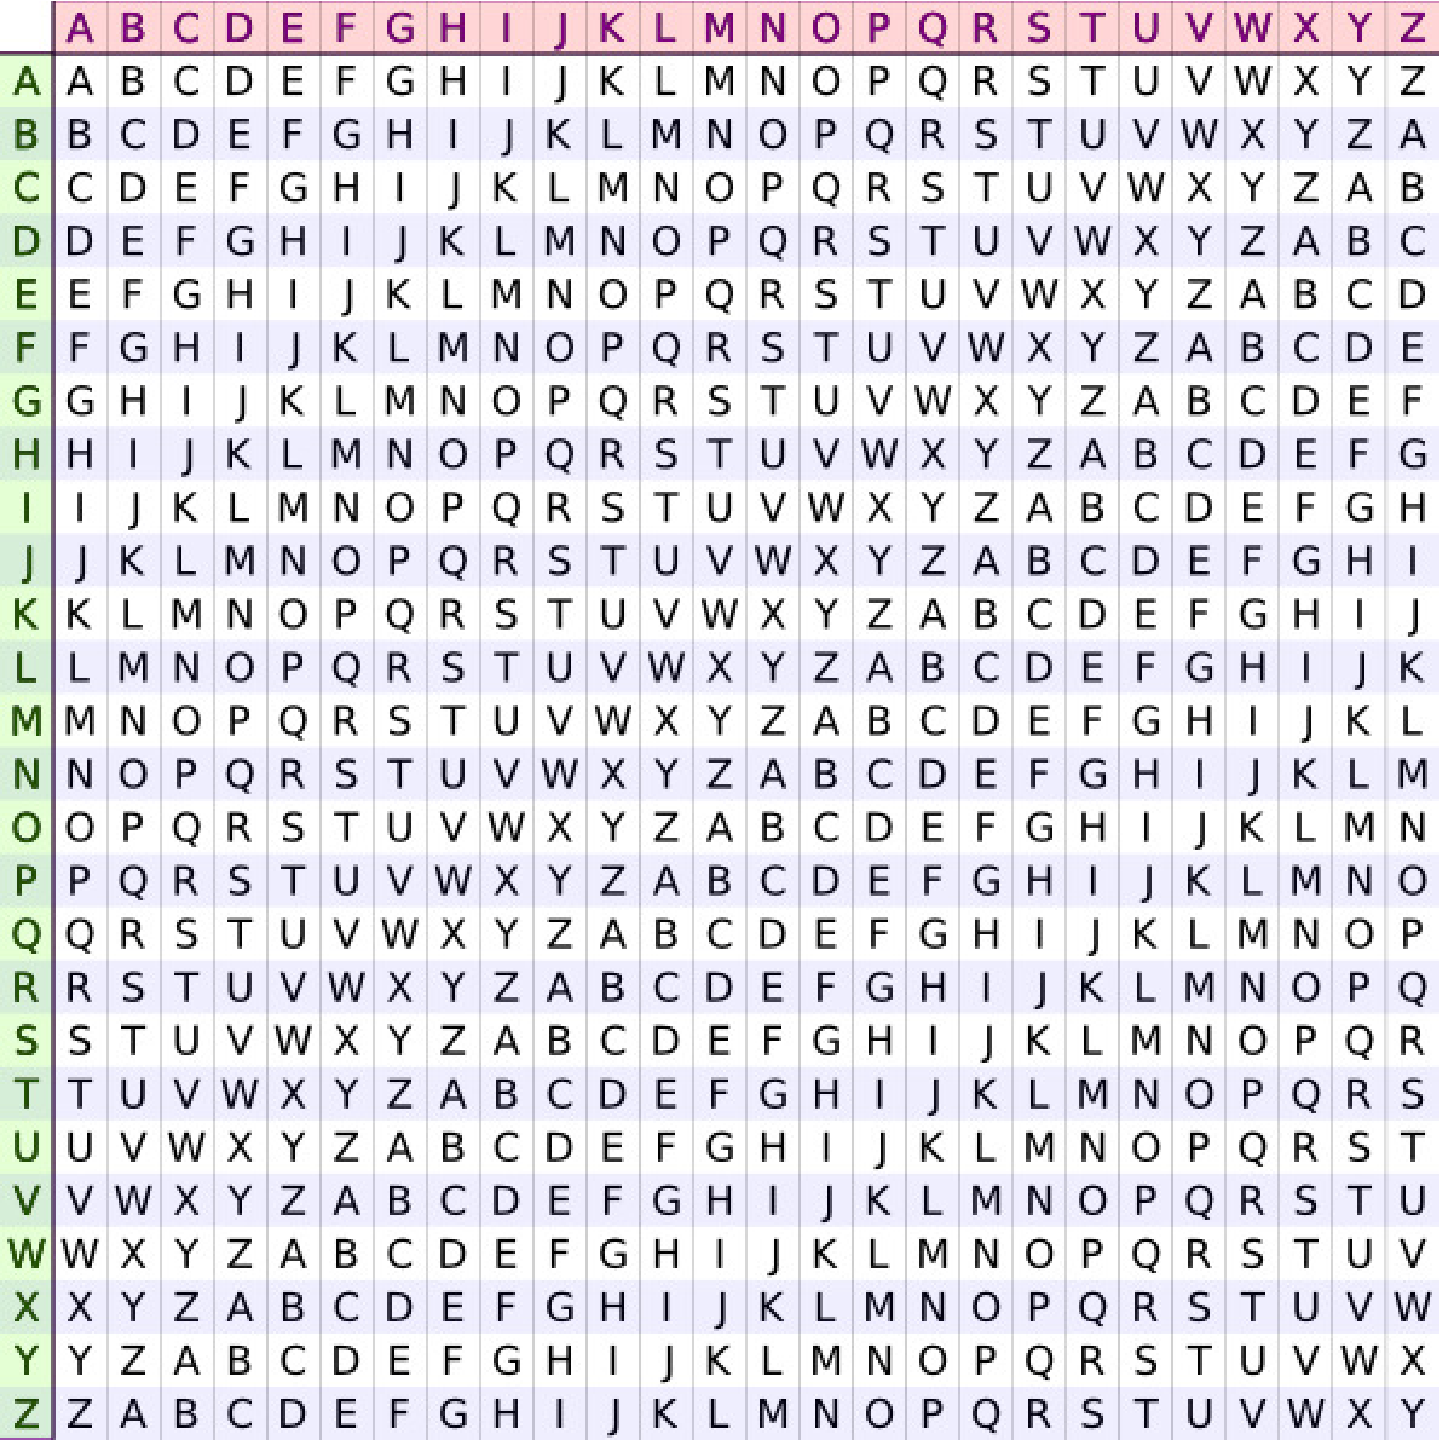
\includegraphics[width=0.95\textwidth]{vigenere.pdf}
	\caption{Table de Vigenère}
	\label{fig:vigenere}
\end{minipage}
\end{figure}




\begin{table}[htbp]
	\centering
		\begin{tabular}{|l|*{25}{|c}|}
		\hline
			mot & a & n & t & i & c & o & n & s & t & i & t & u & t & i & o & n & n & e & l & l & e & m & e & n & t \\
			\hline
			clé & r & o & u & e & r & o & u & e & r & o & u & e & r & o & u & e & r & o & u & e & r & o & u & e & r \\
			\hline
			code & r & b & n & m & t & c & h & w & k & w & n & y & k & w & i & r & e & s & f & p & v & a & y & r & k \\
			\hline
		\end{tabular}
		\caption{Exemple de chiffrement de Vigenère}
		\label{TabVig}
\end{table}


La méthode de chiffrement par lecture de la table est une méthode adaptée \og aux humains\fg, ainsi on réfléchira à l'implémentation d'un algorithme plus efficace en s'aidant de l'exemple.

On dispose de la variable \pyv{alphabet= "abcdefghijklmnopqrstuvwxyz"}. 

On donne le bloc d'instruction suivant : 

\begin{pyverbatim}
alphabet= "abcdefghijklmnopqrstuvwxyz"
for i in range(26):
    alphabet = alphabet[1:]+alphabet[:1]
    print (alphabet)
\end{pyverbatim}

\question{Combien de lignes seront affichées ? Quelles seront les deux premières lignes affichées  ?}

\question{Écrire la fonction \pyv{def generer_table()->list :} qui retourne la table de Vigenère sous la forme d'une liste de listes.}
Le résultat sera de la forme suivante :
\footnotesize{
\begin{pyverbatim}
[['a','b','c','d','e','f','g','h','i','j','k','l','m','n','o','p','q','r','s','t','u','v','w','x','y','z'], 
 ['b','c','d','e','f','g','h','i','j','k','l','m','n','o','p','q','r','s','t','u','v','w','x','y','z','a'],
 ... ]
\end{pyverbatim}
}

\normalsize

On donne deux fonctions permettant de constuire la ligne << clé >> de la table \ref{TabVig} à partir d'un mot et d'une clé. 
\begin{multicols}{2}
\begin{pyverbatim}
1. def generer_cle_1(mot,cle):
2.     nb = len(mot)//len(cle)+1
3.     ch_cle=nb*cle
4.     ch_cle = ch_cle[0:len(mot)]
5.     tab_cle = [car for car in ch_cle]
6.     return tab_cle
\end{pyverbatim}

\begin{pyverbatim}
1. def generer_cle_2(mot,cle):
2.     tab_cle = []
3.     for i in range(len(mot)):
4.         id = i%len(cle)
5.         tab_cle.append(cle[id])
6.     return tab_cle
\end{pyverbatim}

\end{multicols}

\question{En 2 à 3 lignes, expliquer les différences entre les 2 fonctions. Commentez les lignes 2 à 5 des deux fonctions.}

\question{Écrire une fonction étant spécifier ainsi : \pyv{code_vigenere(ch:str, cle:str) -> str } où la chaîne renvoyée correspond à la chaîne codée avec la clé \texttt{cle}. Chaque ligne sera commentée. Vous pourrez utiliser les fonctions définies précédemment.}

%On donne la fonction suivante.
%\begin{lstlisting}
%def decode_vigenere(ch):
%    L = len(cle)
%    alphabet= "abcdefghijklmnopqrstuvwxyz"
%    decode = ""
%    for i in range(len(ch)):
%        d = i
%        while d>L-1:
%            d = d - L
%        index = alphabet.index(ch[i]) - alphabet.index(cle[d])
%        if index < 0 :
%            index = index + N
%        j = alphabet[index]
%        decide = decode + j
%    return decode
%\end{lstlisting}
%%\begin{pyverbatim}
%%def decode_vigenere(ch):
%%\end{pyverbatim}  
%%%    decode=""
%%    for i in range(len(ch)):
%%        d=i
%%        while d>L-1:
%%            d=d-L
%%        index=alphabet.index(ch[i])-alphabet.index(cle[d])
%%        if index<0:
%%            index=index+N
%%        j=alphabet[index]
%%        decode=decode+j
%%    return(decode)
%\question{Écrire une fonction \texttt{decode\_vigenere(chcode,cle)} ayant pour paramètre d'entrée une chaîne de caractères \texttt{chcode}, la clé \texttt{ch} et pour résultat la chaîne \texttt{chcode} décodée : \texttt{chdecode}. }

\question{Quel est selon vous l'intérêt de ce codage par rapport à l'algorithme de César ?}

\vspace{0.5cm}

